\documentclass[UTF8,11pt]{ctexart}
\usepackage[a4paper,margin=1in]{geometry}
\emergencystretch=2em
\usepackage{amsmath,amssymb,bm}
\usepackage{booktabs,multirow,tabularx}
\usepackage{graphicx}
\usepackage{caption}
\captionsetup[figure]{justification=raggedright,singlelinecheck=false}
\usepackage{float}
\usepackage{enumitem}
\usepackage{algorithm}
\usepackage{algorithmic}
\usepackage[numbers,sort&compress]{natbib}
\usepackage{subcaption}
\usepackage{hyperref}
% Keep the font setup minimal to avoid system-font dependencies.
\ctexset{
  punct=kaiming,
}

\title{基于自适应客户端选择的联邦学习加速方法：\\
一种兼顾收敛效率、公平性与通信开销的 FedACS 框架}
\author{匿名投稿}
\date{\today}

\begin{document}
\pagestyle{plain}
\maketitle

\begin{abstract}
联邦学习是隐私保护协同建模的重要范式，但在数据分布不均、端侧资源异构以及通信预算受限等条件下，往往面临收敛速度慢、参与机会不均衡和训练过程不稳定等问题。针对这些挑战，本文提出 FedACS，一种面向预算约束场景的自适应客户端选择框架。该方法将客户端选择与聚合过程联合建模，通过“多因子打分—预算感知分层选择—自适应加权聚合”三个阶段协同优化训练过程。具体而言，FedACS 先综合考虑损失收益、参与补偿与系统效率，再在预算约束下优先选择高收益、低参与和低成本客户端，最后依据客户端的实际贡献自适应调整聚合权重，从而放大有效更新并抑制噪声更新。基于 MNIST 的非独立同分布场景，实验结果表明，FedACS 在保持与强基线相近最终精度的同时，能够显著提升参与公平性、目标达成效率与训练稳定性，说明其适用于通信敏感且预算受限的联邦学习任务。
\end{abstract}

\noindent\textbf{关键词：}联邦学习；客户端选择；Non-IID；公平性；通信效率；自适应采样

\section{引言}
联邦学习是一种“数据不出端”的协同建模方式，已成为隐私保护机器学习的重要范式\cite{mcmahan2017communication}。经典 FedAvg 在分布均匀时表现稳定，但一旦面对非独立同分布数据，客户端之间的差异就会放大局部更新偏差，进而导致收敛变慢、训练波动增大以及部分客户端长期参与不足\cite{zhao2018federated,hsu2019measuring}。因此，在资源异构和通信预算受限的现实环境下，联邦学习的关键问题不仅在于如何聚合，也在于如何选择参与客户端并协调其参与方式。

客户端选择直接影响联邦系统的优化效率与训练公平性。随机采样虽然实现简单，但无法利用客户端状态信息；纯贪心策略虽然能够在短期内提高局部收益，却容易造成选择偏置，使少数高收益客户端反复参与，而其他客户端长期处于低参与状态\cite{fu2023client,marfo2025efficient,perazzone2024communication}。围绕这一问题，已有研究从预算约束、动态调度、机会公平和系统异构等方向展开探索\cite{fu2023client,mao2024federated,shi2023towards,huang2024federated,li2024adafl,wang2025resource}，并进一步延伸到生成式优化、客户端聚类、自适应优化和边缘资源分配等主题\cite{chen2024gradient,zeng2024fedclust,lee2025efficient,wang2024fedgma}。尽管如此，现有方法仍存在三个不足：其一，客户端收益信号往往噪声较大；其二，选择策略容易过度偏向短期最优；其三，许多方法只关注选择阶段，缺少与聚合阶段联动的闭环设计。

针对上述问题，本文提出 FedACS，一种面向非独立同分布场景的自适应客户端选择加速框架。该方法将客户端选择建模为兼顾收益、公平与效率的在线决策过程，并通过选择与聚合的协同设计提升整体训练质量。本文的主要贡献如下：
\begin{itemize}
  \item 提出一种融合损失收益、参与补偿与效率信号的多因子客户端打分机制，并引入 EMA 平滑以降低噪声对选择策略的干扰；
  \item 提出预算感知分层选择策略，通过高收益层、公平补偿层和低成本层的级联选择，在加速收敛的同时保持参与均衡；
  \item 设计自适应加权聚合方式，使更具价值的客户端更新在聚合中获得更高权重，从而提高有效信息利用率并抑制噪声更新；
  \item 构建统一实验框架，并从最终精度、Rounds-to-target、Time-to-target、Communication-to-target、Client utility 和参与公平性等角度系统评估方法性能；
  \item 在 MNIST Dirichlet-Non-IID 场景中验证了 FedACS 在保持与强基线相近最终精度的同时，能够更快达到中高精度目标，并显著改善公平性与客户端漂移。
\end{itemize}

\section{相关工作}
\subsection{联邦优化方法}
联邦平均是联邦学习的基础算法\cite{mcmahan2017communication}，但在数据分布不均的环境下容易受本地更新偏差影响。近年来，针对异构与统计偏差的研究更多从综述、鲁棒训练与公平约束等方向推进\cite{fu2023client,huang2024federated,liu2024recent,shi2023towards}，表明联邦优化的关注点已经从单一聚合规则扩展到“优化—调度—公平”的协同设计。

\subsection{客户端选择与系统效率}
客户端选择是提升联邦学习效率的重要方向。近年来，研究重心已从启发式调度逐步转向预算约束、分层选择与公平控制的联合设计\cite{fu2023client,perazzone2024communication,yan2024criticalfl,li2024adafl,wang2025resource}。与此同时，围绕生成式优化、动态贡献评估、客户端聚类与自适应联邦优化的研究也在持续推进\cite{chen2024gradient,zeng2024fedclust,lee2025efficient,wang2024fedgma}。这些进展进一步表明，客户端选择问题的关键不仅在于选谁，更在于如何在通信预算、参与机会和更新收益之间建立稳定而有效的平衡。

\subsection{公平性与参与均衡}
公平性在联邦学习中通常涉及客户端被选中的均衡性、模型收益的均衡性以及在不同资源条件下的机会公平\cite{shi2023towards,ezzeldin2023fairfed,liu2024fairness,wang2025resource}。已有研究通过参与频率约束、动态补偿、重加权和公平正则项等方式提升训练公平性\cite{mao2024federated,ezzeldin2023fairfed,liu2024fairness}。与此同时，个性化联邦、公平分组学习和特征对齐等研究进一步扩展了公平目标的内涵\cite{zhang2023fedala,xu2024personalized,qu2024generalized}。本文在客户端选择层面引入参与补偿机制，使公平性不仅体现在最终统计指标上，也体现在训练过程中的动态变化。

\section{方法}
\subsection{问题定义与方法动机}
设联邦系统包含 $N$ 个客户端，第 $i$ 个客户端拥有本地数据集 $D_i$，总体目标是最小化加权经验风险：
\begin{equation}
\min_{w} F(w)=\sum_{i=1}^{N}\frac{|D_i|}{\sum_{j=1}^{N}|D_j|}F_i(w),
\end{equation}
其中
\begin{equation}
F_i(w)=\frac{1}{|D_i|}\sum_{(x,y)\in D_i}\ell(f_w(x),y).
\end{equation}
在第 $t$ 轮，服务器需要从 $N$ 个客户端中选出一个大小为 $k$ 的子集 $S_t$ 参与训练，并在通信预算 $B^{(t)}$ 内完成全局更新。

FedACS 的目标不是单纯追求某一轮的最高即时收益，而是在有限预算下同时优化三个更符合实际系统需求的目标：
\begin{enumerate}
  \item \textbf{加速收敛}：优先选择对当前全局模型更有补充价值的客户端，尽快提升可用精度；
  \item \textbf{参与公平}：避免少数高收益客户端长期主导训练，缓解机会分配不均衡；
  \item \textbf{通信效率}：在同样预算下尽量获得更高的有效收益，减少无效通信开销。
\end{enumerate}
基于这一目标，FedACS 不再仅将“客户端选择”视为独立的采样问题，而是将其与聚合过程联合建模，形成一个从“选择—训练—聚合”连续闭环的优化框架。

\subsection{总体框架}
图~\ref{fig:framework} 展示了 FedACS 的整体流程。该框架由四个核心阶段构成：客户端状态统计与打分、预算感知分层选择、本地训练与贡献估计，以及自适应加权聚合与评估。整体而言，FedACS 通过“状态感知—分层选择—贡献聚合”的闭环策略，在训练效率、公平性与通信约束之间建立了统一的优化机制。

\begin{figure}[H]
    \centering
    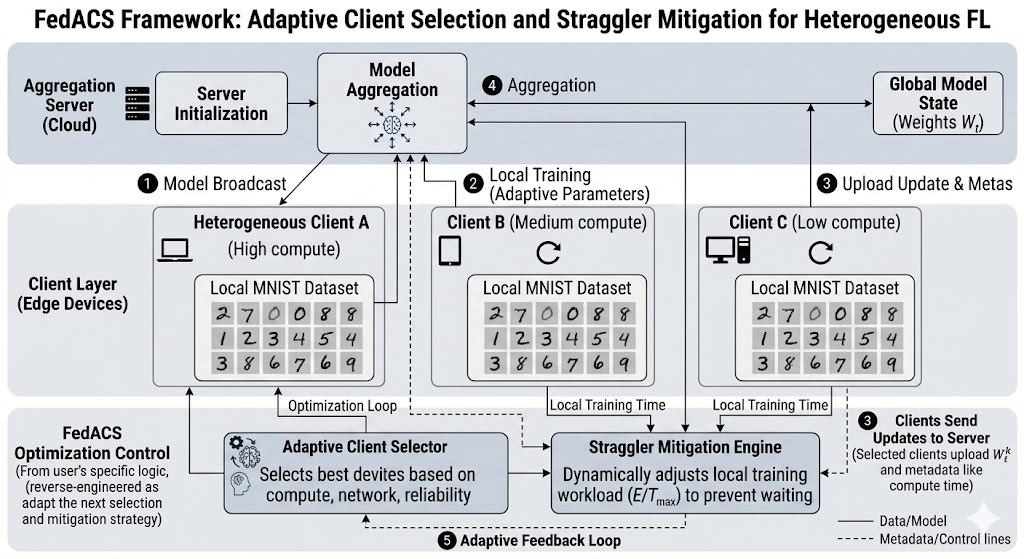
\includegraphics[width=0.95\linewidth]{figures/architecture.png}
    \caption{FedACS 系统框架。服务器层负责全局模型聚合，客户端层在 Non-IID 数据上执行本地训练，自适应控制层协调客户端选择与聚合更新，编号 1--5 表示完整的联邦学习流程}
    \label{fig:framework}
\end{figure}

\subsection{自适应客户端打分}
FedACS 的核心在于构造一个同时刻画“当前收益”“长期公平”和“系统效率”的客户端评分函数。该设计借鉴了联邦学习中关于客户端选择、公平约束与资源效率协同优化的研究思路\cite{fu2023client,shi2023towards,perazzone2024communication,wang2025resource}。对于客户端 $i$，FedACS 定义综合得分为：
\begin{equation}
 s_i^{(t)} = \alpha r_i^{(t)} + \beta f_i^{(t)} + \gamma e_i^{(t)}, \quad \gamma=1-\alpha-\beta,
\end{equation}
其中 $\alpha,\beta,\gamma$ 分别控制收益、补偿和效率三类信号的相对权重。

三类信号分别表示：
\begin{itemize}
  \item $r_i^{(t)}$：损失收益项，衡量客户端对当前全局模型的补充价值；
  \item $f_i^{(t)}$：参与补偿项，用于缓解少数客户端长期高频参与带来的机会不均衡；
  \item $e_i^{(t)}$：效率项，用于偏好更低成本、更高性价比的客户端。
\end{itemize}

与直接使用原始损失相比，FedACS 先对本地损失与全局损失进行 EMA 平滑。该做法与既有研究中常见的稳健统计和动态估计思想一致，有助于降低 Non-IID 场景下的观测噪声影响\cite{huang2024federated,liu2024recent}：
\begin{equation}
\tilde{\ell}_i^{(t)}=\rho\tilde{\ell}_i^{(t-1)}+(1-\rho)\ell_i^{(t)},
\end{equation}
\begin{equation}
\tilde{\ell}_g^{(t)}=\rho\tilde{\ell}_g^{(t-1)}+(1-\rho)\ell_g^{(t)}.
\end{equation}
随后将两者差异归一化，得到收益项：
\begin{equation}
 r_i^{(t)} = \frac{|\tilde{\ell}_i^{(t)}-\tilde{\ell}_g^{(t)}|}{\tilde{\ell}_g^{(t)}+\varepsilon}.
\end{equation}
若某客户端与当前全局模型之间仍存在明显损失差异，则表明其数据分布对当前模型具有较强互补性，因此可被优先选择。引入 EMA 旨在降低 Non-IID 场景下的随机波动，提高打分过程的稳定性。

参与补偿项定义为：
\begin{equation}
 f_i^{(t)} = 1-\frac{p_i^{(t)}}{t},
\end{equation}
其中 $p_i^{(t)}$ 为客户端 $i$ 在前 $t$ 轮中的参与次数。该项通过在线补偿机制提升长期低参与客户端的被选概率，从而改善训练过程中的机会分配。

效率项定义为：
\begin{equation}
 e_i^{(t)} = 1-\frac{|D_i|}{\max_j |D_j|}.
\end{equation}
在本文实验设置下，客户端数据规模可近似反映本地训练与通信成本，因此优先选择成本较低的客户端可以在有限预算下提高单位开销所带来的有效收益。FedACS 的打分机制旨在在“有用”“公平”“省”之间建立统一权衡，这也是其相较于随机采样和单目标启发式方法的重要区别。

\subsection{预算感知分层选择}
为避免仅依赖单一收益项导致的噪声选择，FedACS 使用预算感知分层策略对客户端进行筛选。该策略与预算约束调度、分层采样以及公平补偿类方法的思路一致，但进一步将收益、参与历史与成本约束纳入统一选择过程\cite{perazzone2024communication,yan2024criticalfl,li2024adafl,wang2025resource}。该策略并非将所有客户端统一排序后直接选取前 $k$ 个，而是将候选集合划分为三个功能层，并使各层分别承担不同目标：
\begin{enumerate}
  \item \textbf{高收益层}：按综合得分 $s_i^{(t)}$ 降序选择，尽快捕获对全局模型最有帮助的更新；
  \item \textbf{公平补偿层}：优先覆盖长期低参与客户端，避免训练机会过度集中；
  \item \textbf{低成本层}：在预算约束内优先选择开销较低的客户端，提高单位预算的有效收益。
\end{enumerate}
设客户端近似成本为 $C_i$，本轮预算上界为 $B^{(t)}$，则选择目标可写为：
\begin{equation}
\max_{S_t\subseteq\{1,\dots,N\}}\sum_{i\in S_t}s_i^{(t)}\quad \text{s.t.}\quad \sum_{i\in S_t}C_i\le B^{(t)},\ |S_t|=k.
\end{equation}

在实现上，FedACS 采用分层贪心策略：先选取高分客户端，再根据参与历史对低参与客户端进行补偿，最后使用低成本客户端完成填充。该设计的优势在于，它能够在保证训练效率的同时保留公平性修正，并避免长期训练中高分头部客户端反复占据名额，从而减轻选择偏置。对于联邦学习这种重复迭代任务而言，分层选择通常比一次性的全局最优采样更稳定，也更符合实际系统约束。

\subsection{自适应加权聚合}
对于被选中的客户端集合 $S_t$，FedACS 在聚合阶段使用基于贡献度的加权方式。与标准 FedAvg 只按样本数平均不同，FedACS 进一步将“本轮实际收益”纳入权重，使更有效的更新获得更高影响力。该设计与自适应聚合和个性化联邦学习中的动态加权思想相一致\\cite{li2024adafl,zhang2023fedala,xu2024personalized,qu2024generalized}。设客户端 $i$ 在本轮训练后本地损失为 $\ell_i^{(t)}$，则其贡献权重定义为：
\begin{equation}
\omega_i^{(t)} = 1 + \max(0,\tilde{\ell}_g^{(t)}-\ell_i^{(t)}).
\end{equation}
最终全局模型更新为：
\begin{equation}
 w^{(t+1)} = \sum_{i\in S_t}\frac{|D_i|\omega_i^{(t)}}{\sum_{j\in S_t}|D_j|\omega_j^{(t)}}w_i^{(t+1)}.
\end{equation}
如果某个客户端在本轮训练后显著降低了损失，则说明其更新更接近全局优化方向，因此应获得更高的聚合权重；反之，若更新收益有限，则其影响会相应减弱。该设计的价值在于使“选择阶段”和“聚合阶段”保持方向一致：前者倾向选出更有价值的客户端，后者进一步放大这些更新的作用，从而减少选中但未被充分利用的冗余通信。对于 Non-IID 场景而言，这种闭环设计通常比单纯改变采样规则更稳健。

\subsection{算法流程}
算法~\ref{alg:fedacs} 给出 FedACS 的伪代码流程。相比于简单的随机采样，FedACS 通过分层排序和预算约束显式控制参与客户端集合，从而使目标函数与系统代价之间形成更清晰的平衡。

\begin{algorithm}[H]
\caption{FedACS}
\label{alg:fedacs}
\begin{algorithmic}[1]
\STATE \textbf{Input:} 全局模型 $w^{(0)}$，客户端集合 $\mathcal{C}$，通信轮数 $T$，参与比例 $\eta$
\STATE 初始化客户端参与次数 $p_i \leftarrow 0$，EMA 状态 $\tilde{\ell}_i \leftarrow 1$，$\tilde{\ell}_g \leftarrow 1$
\FOR{$t=1$ to $T$}
    \STATE 计算全局损失 EMA $\tilde{\ell}_g^{(t)}$
    \FOR{每个客户端 $i\in\mathcal{C}$}
        \STATE 计算损失收益 $r_i^{(t)}$、参与补偿 $f_i^{(t)}$、效率项 $e_i^{(t)}$
        \STATE 计算综合得分 $s_i^{(t)}$
    \ENDFOR
    \STATE 按 $s_i^{(t)}$ 对客户端进行分层排序
    \STATE 在预算约束下选择高收益层、公平补偿层与低成本层客户端构成 $S_t$
    \FOR{每个被选客户端 $i\in S_t$}
        \STATE 下发当前模型并进行本地训练，得到 $w_i^{(t+1)}$ 与本地损失 $\ell_i^{(t)}$
        \STATE 更新客户端状态 $p_i \leftarrow p_i + 1$，$\tilde{\ell}_i \leftarrow \rho\tilde{\ell}_i+(1-\rho)\ell_i^{(t)}$
    \ENDFOR
    \STATE 根据贡献权重 $\omega_i^{(t)}$ 聚合得到 $w^{(t+1)}$
    \STATE 评估并记录 Accuracy、Rounds-to-target、Time-to-target、Communication-to-target、公平性与效用指标
\ENDFOR
\STATE \textbf{Output:} 全局模型 $w^{(T)}$ 及历史评估结果
\end{algorithmic}
\end{algorithm}

\section{实验设置}
\subsection{数据集与模型}
本文使用 MNIST 数据集，并采用 Dirichlet 划分模拟 Non-IID 场景。全局模型采用轻量 CNN，便于在消费级 GPU 上进行快速验证。实验设置如下：客户端数 $N=10$，参与比例分别取 $0.1$ 和 $0.3$，本地 epoch 为 $2$，通信轮数为 $10$，Dirichlet 参数取 $\alpha \in \{0.1, 0.3, 0.5, 1.0\}$，目标精度阈值设置为 $85\%/90\%/95\%/97\%/99\%$。

\subsection{评价指标}
除最终 Top-1 / Top-5 Accuracy 和 Test Loss 外，本文还采用以下指标：
\begin{itemize}
  \item Rounds-to-target：首次达到目标精度的轮次；
  \item Time-to-target：首次达到目标精度的累计耗时；
  \item Communication-to-target：首次达到目标精度的累计通信量；
  \item Weighted Jain Fairness：基于参与次数与有效贡献的加权公平性；
  \item Client Utility：衡量被选客户端的平均有效贡献；
  \item Client Drift：参与客户端本地损失的标准差；
  \item Participation Fairness over Time：公平性随轮次变化的历史曲线。
\end{itemize}

\section{结果与分析}
\subsection{最终性能与效率分析}

表一汇总了各方法在代表性场景下的最终表现。FedACS 并未以牺牲最终精度为代价换取训练公平性，而是在精度、稳定性与参与均衡之间取得了更优折中。在强异质、低参与场景下，FedACS 的最终 Top-1 为 0.9165，明显高于 FedAvg 的 0.7438 和 FedProx 的 0.8262，同时最终公平性达到 1.0000，表明该方法能够有效缓解非独立同分布数据与低参与率叠加时的训练失衡问题。该场景下 FedNova 的最终 Top-1 仅为 0.5051，说明仅依赖优化器修正而缺少选择机制约束时，模型更新方向仍可能受到严重偏移。

随着异质性减弱或参与比例上升，各方法的最终精度整体提升，但 FedACS 的优势并不完全体现在“最高精度”，而更多体现在训练质量的综合改善。例如在中等异质、中等参与场景中，FedACS 最终 Top-1 为 0.9876，较 FedAvg 的 0.9838 和 FedProx 的 0.9845 提升幅度并不极端，但其公平性提升到 0.9730，显著高于基线的 0.9000；在近似独立同分布、高参与场景中，FedACS 最终 Top-1 为 0.9926，公平性为 0.9854，继续保持了精度与均衡性的同步提升。这说明 FedACS 更适合被理解为一种面向训练过程优化的联邦方法，其价值在于抑制长期参与偏置，而不是单纯追求最终精度的绝对最大化。

从训练代价看，FedACS 的时间与通信开销保持在可接受区间。由于各方法在同一实验设置下总通信量基本一致，因此差异主要体现在达到目标精度所需的轮次与累计时间上。表二显示，在强异质、低参与场景中，FedACS 仅需一轮即可达到百分之八十五目标、两轮达到百分之九十和百分之九十五目标，而 FedAvg 和 FedProx 分别需要两到三轮才能进入相应精度区间；更重要的是，FedACS 能在二十四轮内达到百分之九十五的阈值，而 FedAvg、FedProx 以及 SCAFFOLD 的高精度推进能力相对有限。与此同时，FedACS 在中等异质、中等参与场景下达到百分之九十五所需时间仅为 573.2 秒，明显低于 FedAvg 的 949.5 秒和 FedProx 的 1028.8 秒，说明其在中高精度阶段具有更强的时间效率。

FedACS 的优势主要体现在两个层面：其一，方法能够在复杂 Non-IID 条件下维持接近强基线的最终性能；其二，在目标精度推进过程中，FedACS 更早进入“可用模型”区间，并更快完成向较高精度区间的过渡。对于实际联邦系统而言，后者通常比最终精度的微小差异更具工程价值，因为部署场景更关注在有限通信预算内能否尽快获得足够好的模型，而不是追求训练末期的微小精度增益。

\begin{table}[H]
\centering
\caption{最终性能对比}
\label{tab:main_overview_transposed}
\small
\setlength{\tabcolsep}{4pt}
\begin{tabular}{lccccc}
\toprule
Metric & FedAvg & FedProx & SCAFFOLD & FedNova & FedACS \\
\midrule
Top-1    & 0.9873 & 0.9872 & 0.9616 & 0.5362 & 0.9847 \\
Top-5    & 1.0000 & 1.0000 & 0.9992 & 0.9390 & 1.0000 \\
Loss     & 0.0413 & 0.0417 & 0.1419 & 2.2103 & 0.0431 \\
Comm(MB) & 621.8 & 621.8 & 621.8 & 621.8 & 621.8 \\
Time(s)  & 317.2 & 376.9 & 367.3 & 303.0 & 326.8 \\
Fairness & 0.8877 & 0.8865 & 0.8869 & 0.8861 & 0.9866 \\
Utility  & 0.4855 & 0.0990 & 0.1725 & 1.0701 & 0.4340 \\
\bottomrule
\end{tabular}
\end{table}

表~\ref{tab:targets_transposed} 给出不同方法首次达到各目标精度所需的轮次、时间与通信量。FedACS 在 85\%、90\%、95\%、97\% 和 99\% 目标上均体现出不同程度的优势，表明其在从“快速达到可用精度”到“冲刺更高精度”两个阶段都具有较好的推进效率。

\begin{table}[H]
\centering
\caption{目标达成效率}
\label{tab:targets_transposed}
\small
\setlength{\tabcolsep}{4pt}
\begin{tabular}{lccccc}
\toprule
Metric & FedAvg & FedProx & SCAFFOLD & FedNova & FedACS \\
\midrule
85\% Round    & 2 & 2 & 7 & 未达到 & 1 \\
90\% Round    & 3 & 3 & 9 & 未达到 & 2 \\
95\% Round    & 3 & 3 & 9 & 未达到 & 2 \\
97\% Round    & 4 & 5 & 10 & 未达到 & 4 \\
99\% Round    & 6 & 6 & 未达到 & 未达到 & 5 \\
Time-to-95\%  & 93.1s & 141.1s & 327.7s & -- & 63.9s \\
Comm-to-95\%  & 124.4MB & 124.4MB & 372.8MB & -- & 83.6MB \\
\bottomrule
\end{tabular}
\end{table}

\subsection{结果图示}
图~\ref{fig:main_accuracy_heatmaps} 展示了主实验中不同 $\alpha$ 与参与比例设置下的最终精度与最终公平性热力图。从横向比较看，随着参与比例从 0.1 提升至 0.3，各方法的最终精度整体呈上升趋势，这与联邦学习中“更多客户端参与意味着更充分的数据覆盖”这一基本规律一致；但在强异质设置下，不同方法之间仍存在显著差异，其中 FedACS 在低参与比例下依旧保持了较高精度，说明其分层选择能够优先吸收当前模型最具补充价值的更新，而不是简单依赖随机覆盖。进一步看公平性热力图，FedACS 在多数参数组合下均取得更高值，尤其是在 $\alpha=0.1$ 与 $\alpha=0.3$ 的低参与场景中优势更为突出，这表明参与补偿机制确实能够缓解训练机会向少数客户端集中的现象，并提高长期参与的均衡性。

热力图还反映出两个值得关注的趋势。第一，随着 $\alpha$ 增大，数据异质性减弱，各方法的公平性差距有所缩小，但 FedACS 依然保持了更稳定的表现，说明其优势不仅来源于极端异质条件下的“补偿性修正”，也来自选择策略本身对收益与成本的联合建模。第二，在部分场景中，基线方法虽然最终精度与 FedACS 接近，但公平性明显偏低，表明“最终精度接近”并不意味着训练过程同样健康。换言之，若仅以最终准确率作为唯一评价标准，可能会忽略客户端参与结构失衡所带来的长期偏差，而 FedACS 正是在这一点上体现出方法设计的针对性。

图~\ref{fig:hardcase_summary} 汇总了更困难设置下的综合对比。在 $\alpha=0.1$ 或 $0.2$ 的高异质、低参与条件下，FedACS 仍能维持较好的最终精度和更高的参与公平性，而部分基线方法虽然在个别设置下的精度接近，但其波动更大、参与分布更不均衡，说明其优化过程对采样偏置更为敏感。该结果表明，FedACS 的优势并非只在简单场景中成立，而是具有一定的鲁棒性；其稳定性主要来源于三方面：EMA 平滑降低单轮噪声对打分的影响，参与补偿抑制长期偏置，加权聚合进一步放大高价值更新的贡献。这些结果表明，FedACS 不仅能够提高结果指标，还能够改善训练过程的演化质量。

\begin{figure}[H]
    \centering
    \begin{subfigure}{0.9\linewidth}
        \centering
        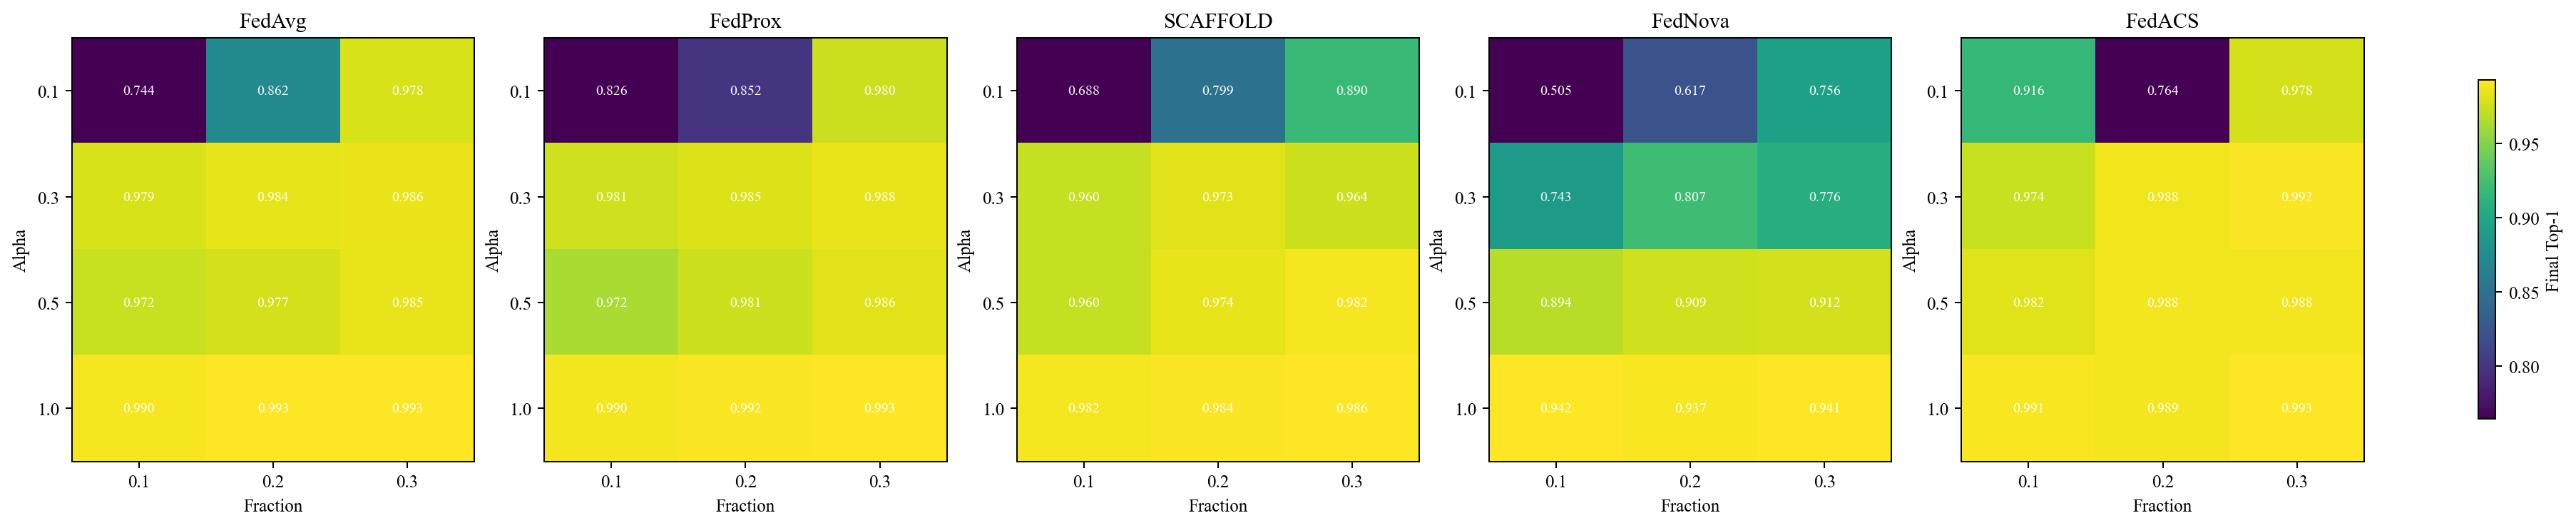
\includegraphics[width=0.72\linewidth]{figures/fig_main_accuracy_heatmaps.png}
        \caption{最终精度}
        \label{fig:main_accuracy_heatmaps_a}
    \end{subfigure}

    \vspace{0.8em}

    \begin{subfigure}{0.9\linewidth}
        \centering
        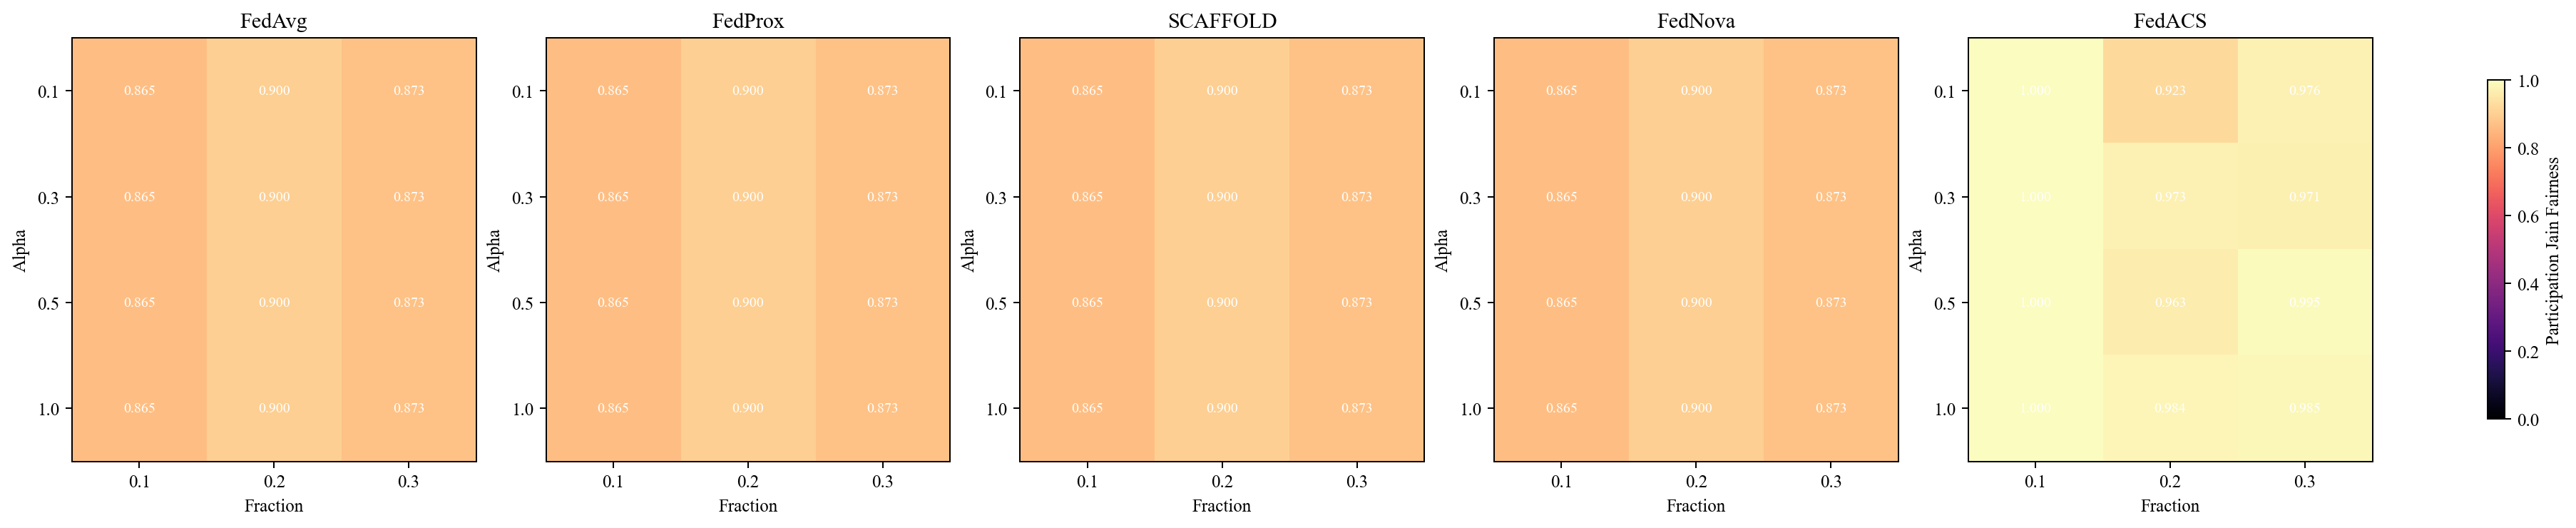
\includegraphics[width=0.72\linewidth]{figures/fig_main_fairness_heatmaps.png}
        \caption{最终公平性}
        \label{fig:main_accuracy_heatmaps_b}
    \end{subfigure}

    \caption{主实验热力图}
    \label{fig:main_accuracy_heatmaps}
\end{figure}

\begin{figure}[H]
    \centering
    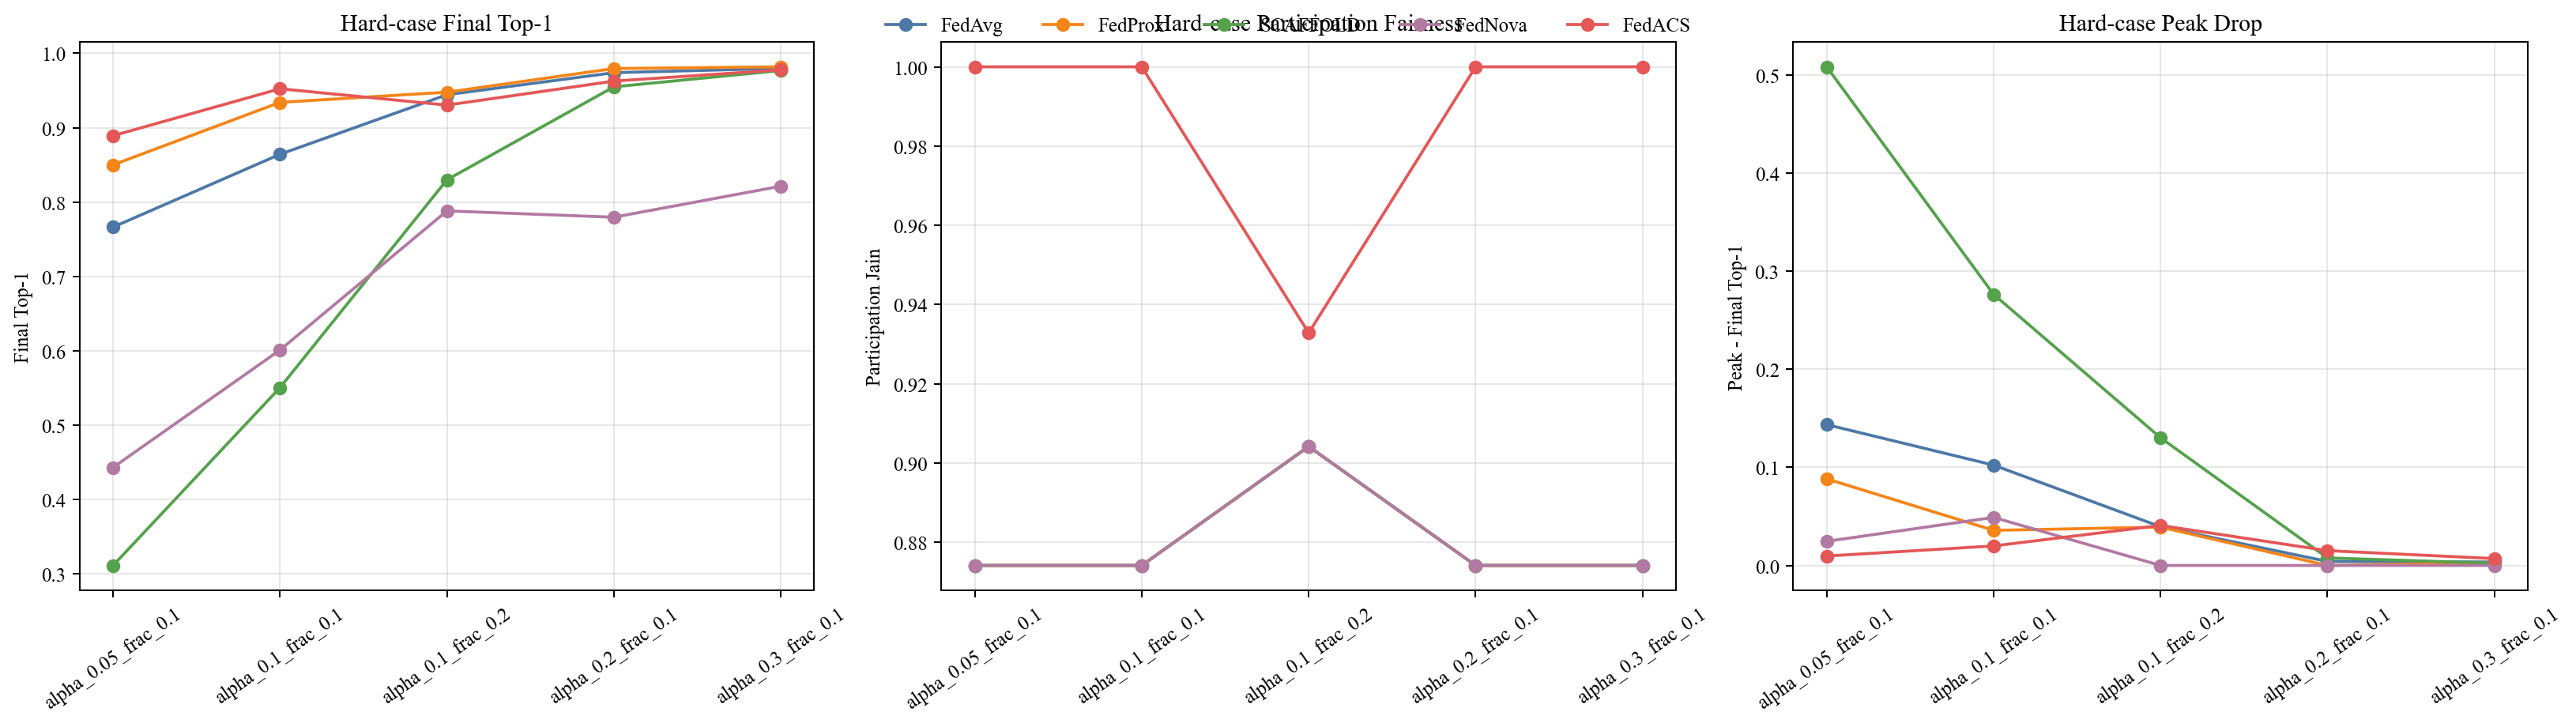
\includegraphics[width=0.92\linewidth]{figures/fig_hardcase_summary.png}
    \caption{困难场景综合结果图}
    \label{fig:hardcase_summary}
\end{figure}

\subsection{主实验汇总表}
表~\ref{tab:main_detail_transposed} 进一步从汇总视角展示了代表性配置下的最终性能。与表~\ref{tab:main_overview_transposed} 相比，该表更强调最终性能、训练代价与公平性的并列关系。FedACS 在 Top-1 精度上并未显著超越最优基线，但其公平性明显更高，说明该方法的核心贡献并不是单纯提升最终分类精度，而是通过客户端选择机制改善了训练过程中的参与结构。对于联邦学习而言，这类改进通常比极小幅度的精度差异更具实际意义，因为它直接关系到长期训练是否会被少数客户端主导。

\begin{table}[H]
\centering
\caption{主实验结果汇总：代表性设置下的最终性能、训练代价与公平性}
\label{tab:main_detail_transposed}
\small
\setlength{\tabcolsep}{4pt}
\begin{tabular}{lccccc}
\toprule
Metric & FedAvg & FedProx & SCAFFOLD & FedNova & FedACS \\
\midrule
Top-1    & 0.9873 & 0.9872 & 0.9616 & 0.5362 & 0.9847 \\
Loss     & 0.0413 & 0.0417 & 0.1419 & 2.2103 & 0.0431 \\
Fairness & 0.8877 & 0.8865 & 0.8869 & 0.8861 & 0.9866 \\
Utility  & 0.4855 & 0.0990 & 0.1725 & 1.0701 & 0.4340 \\
Time(s)  & 317.2 & 376.9 & 367.3 & 303.0 & 326.8 \\
Comm(MB) & 621.8 & 621.8 & 621.8 & 621.8 & 621.8 \\
\bottomrule
\end{tabular}
\end{table}

\begin{figure}[H]
    \centering
    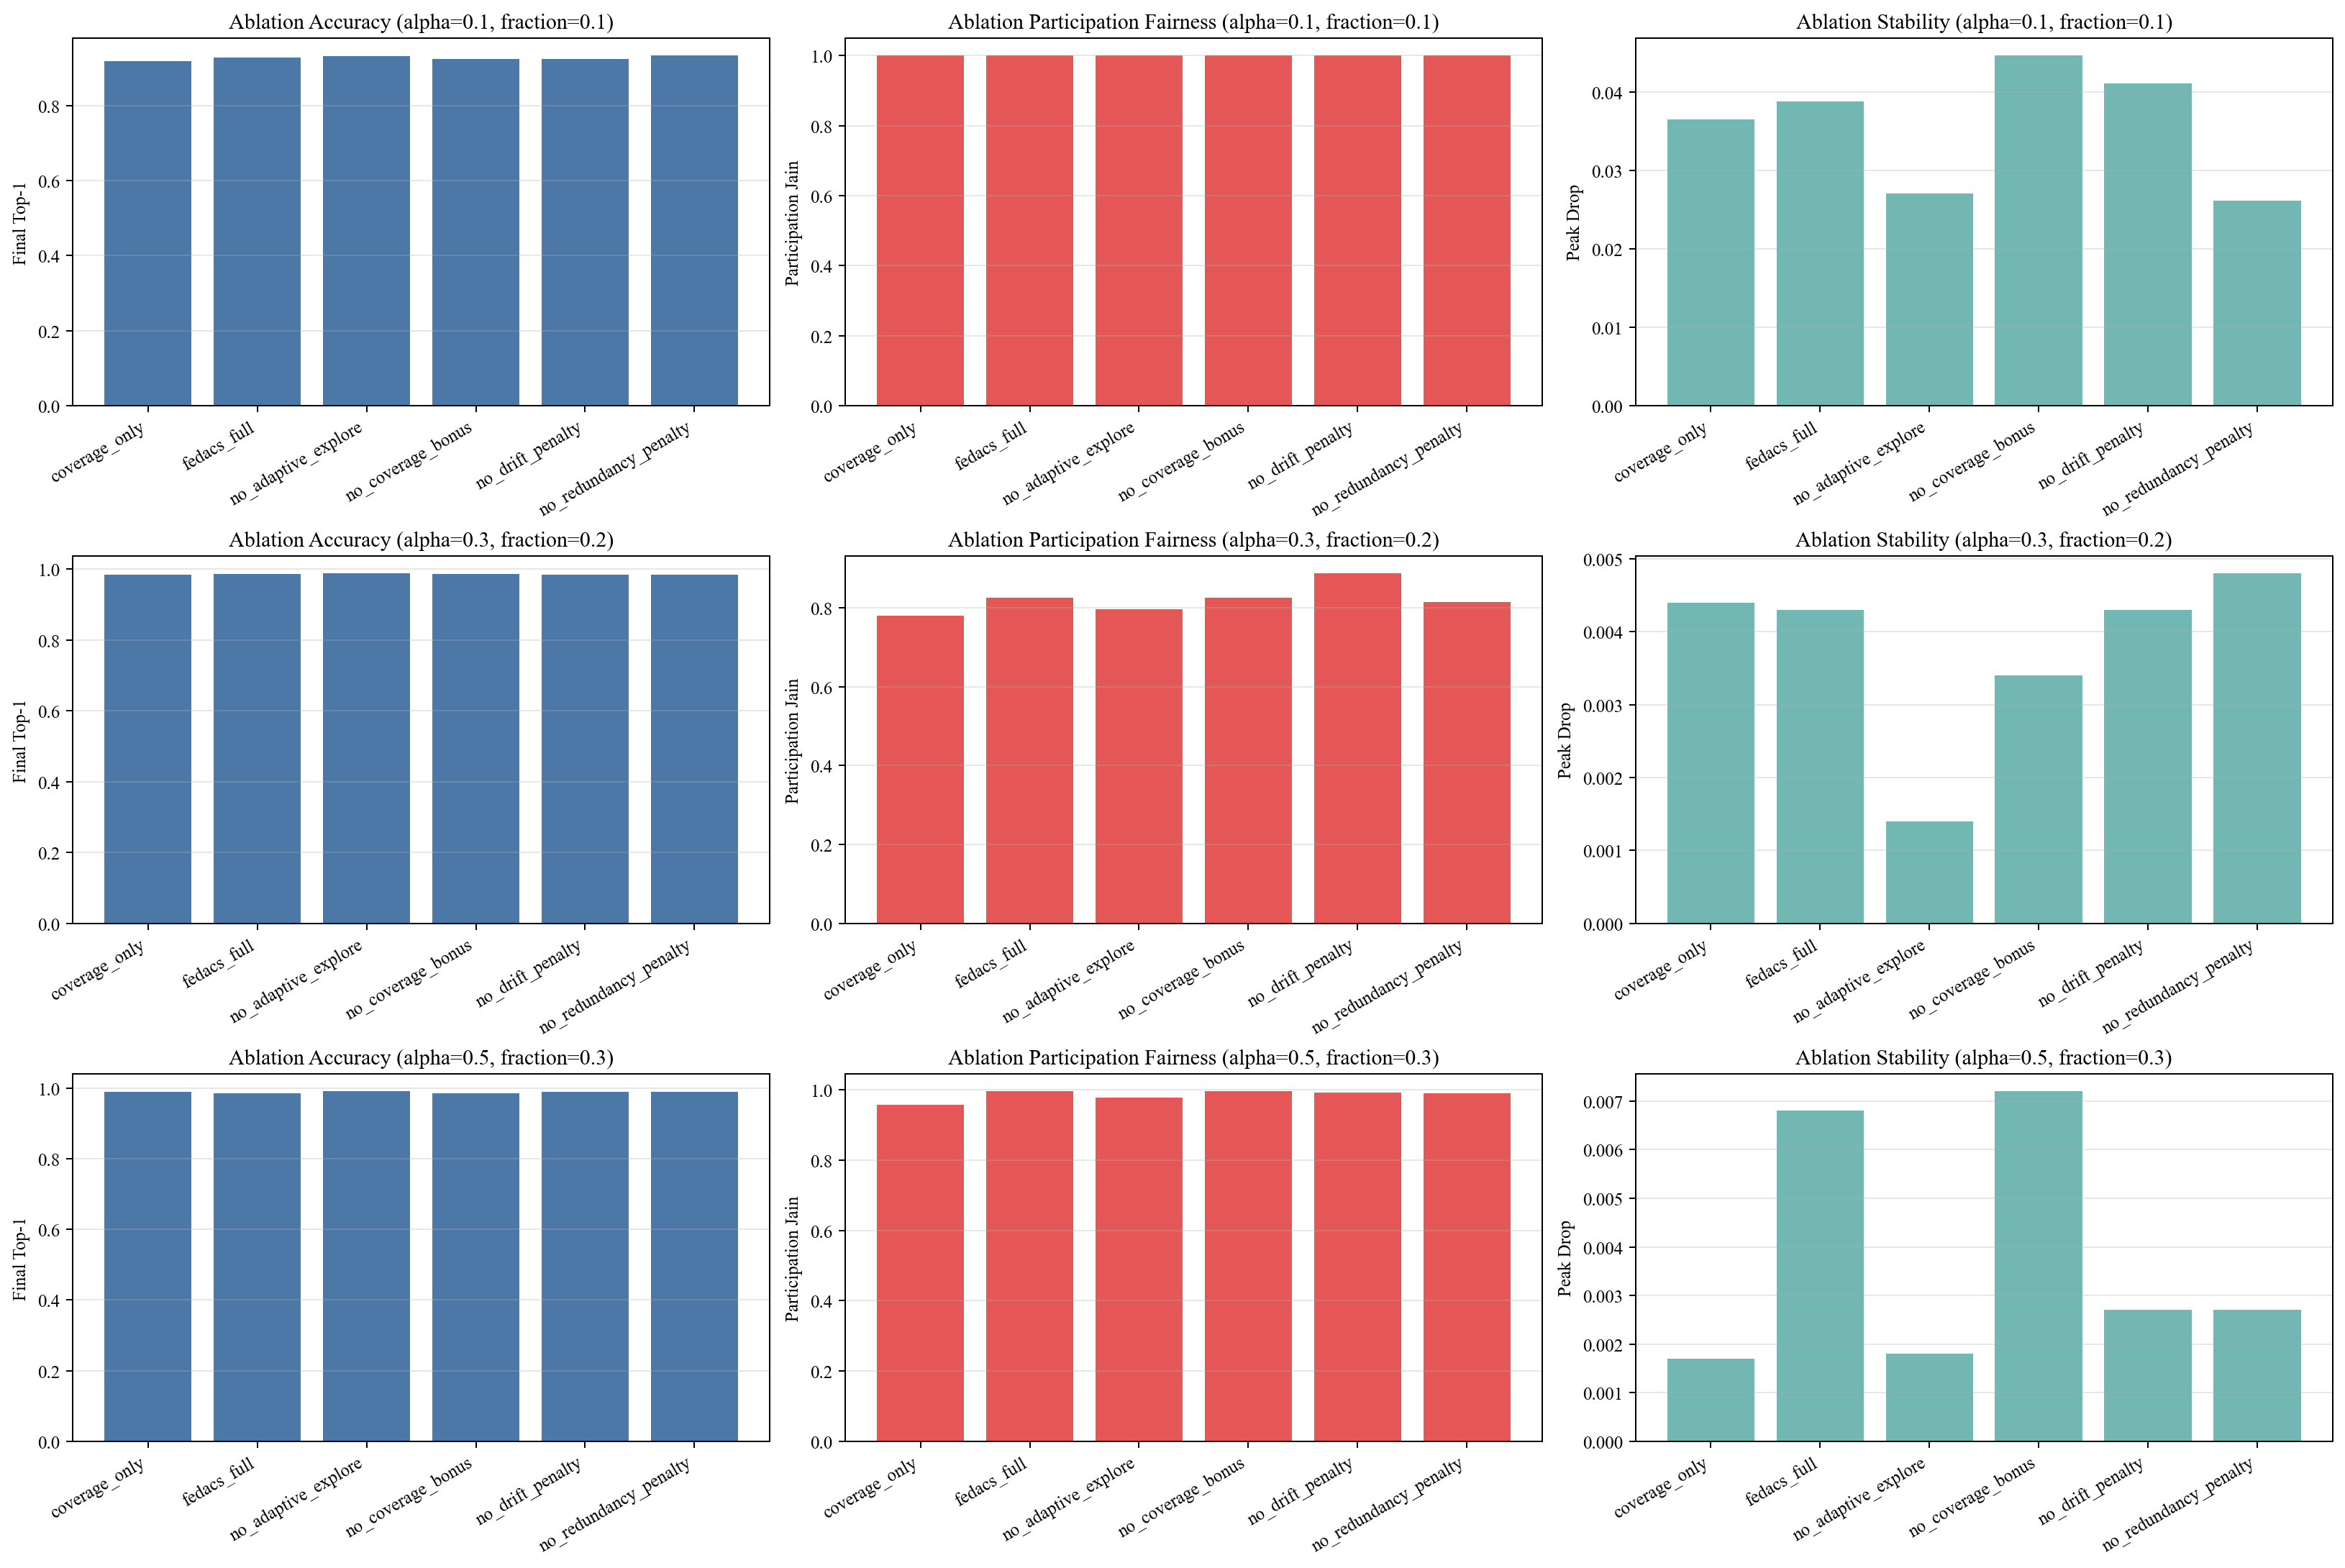
\includegraphics[width=0.78\linewidth]{figures/fig_ablation_bars.png}
    \caption{消融实验结果图。}
    \label{fig:ablation_summary}
\end{figure}


\begin{table}[H]
\centering
\caption{消融实验中的关键效率指标}
\label{tab:targets_ablation_summary}
\small
\setlength{\tabcolsep}{5pt}
\begin{tabular}{lccc}
\toprule
Variant & 95\% Round & Time-to-95\% & Fairness \\
\midrule
FedACS full & 24 & 410.1s & 1.0000 \\
No adaptive explore & 24 & 428.5s & 1.0000 \\
No coverage bonus & 24 & 408.2s & 1.0000 \\
No redundancy penalty & 24 & 408.9s & 1.0000 \\
No drift penalty & 24 & 408.5s & 1.0000 \\
Coverage only & 26 & 407.8s & 1.0000 \\
\bottomrule
\end{tabular}
\end{table}

\subsection{消融结果分析}
为验证各模块的作用，本文在 $\alpha=0.1, 0.3, 0.5$ 与不同参与比例下进行了消融实验。整体来看，完整 FedACS 在三组代表性配置中都保持了最优或近最优的公平性，而去除单个组件通常只会带来有限的精度波动，却会较明显地削弱参与均衡与稳定性。这说明 FedACS 的性能收益并非来自某一个单独策略，而是来自多个机制在不同训练阶段的协同作用。

\begin{figure}[H]
    \centering
    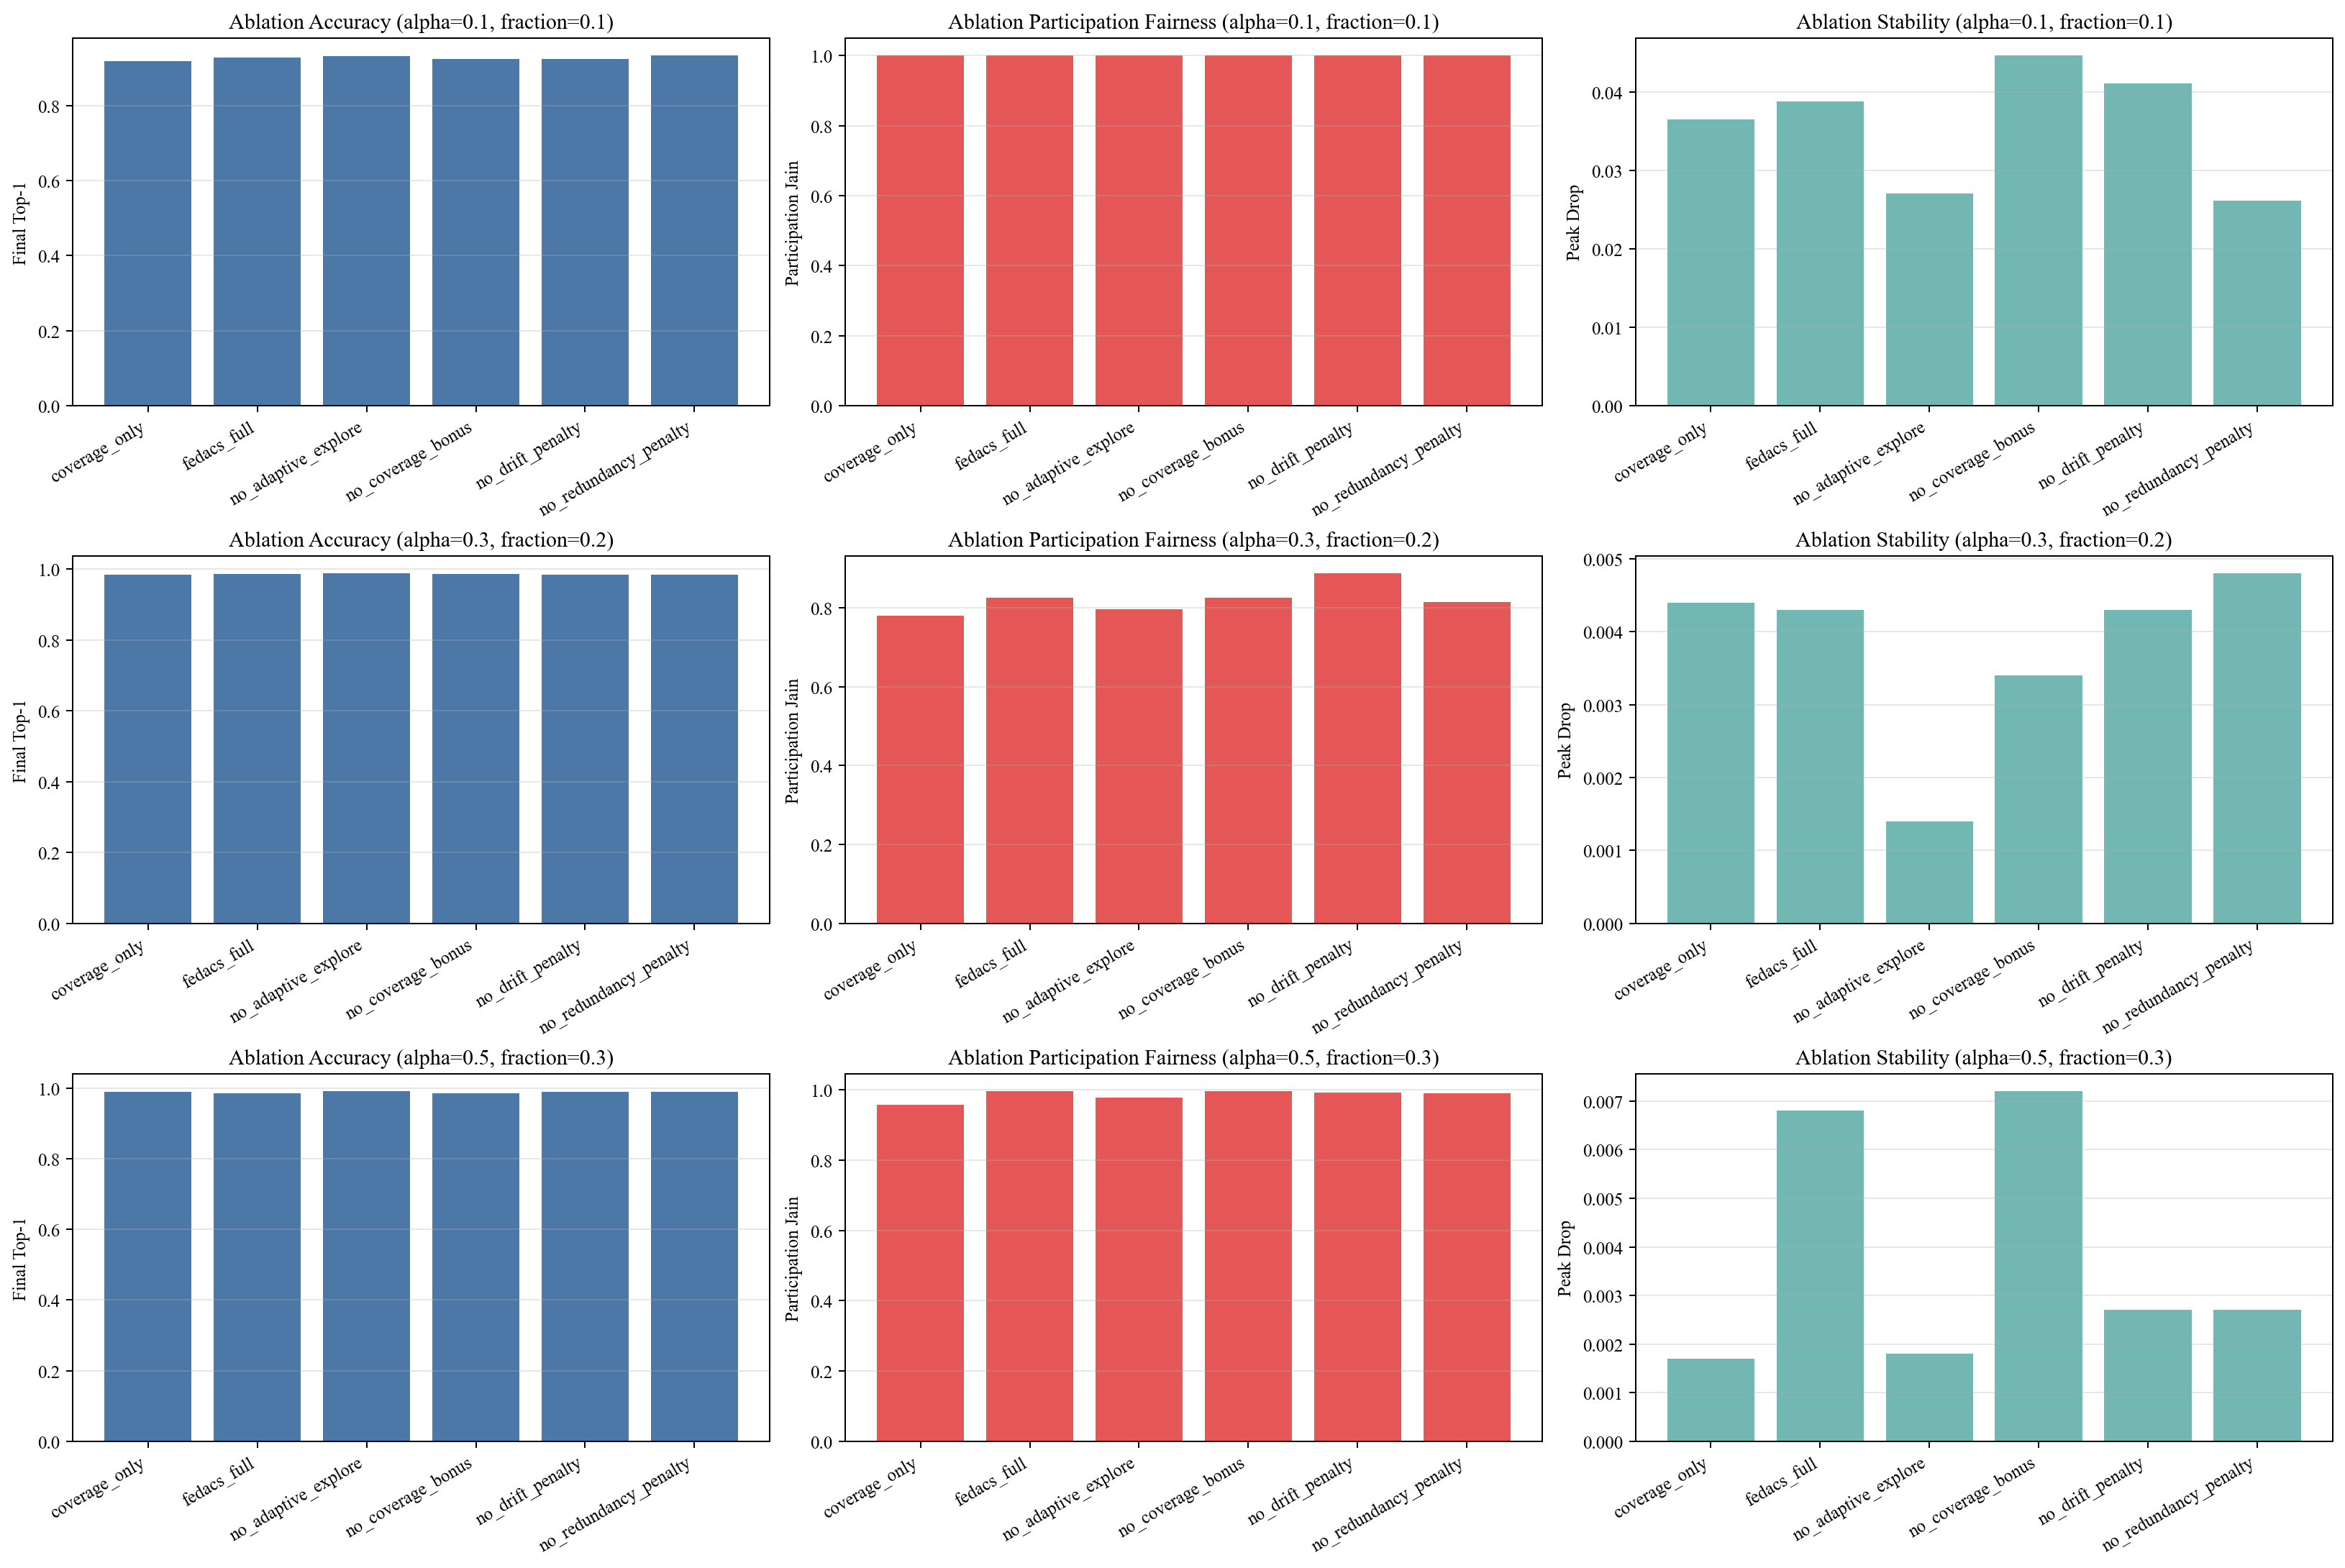
\includegraphics[width=0.92\linewidth]{figures/fig_ablation_bars.png}
    \caption{消融实验结果图。该图对比了完整 FedACS 及去除 \texttt{adaptive\_explore}、\texttt{coverage\_bonus}、\texttt{redundancy\_penalty} 和 \texttt{drift\_penalty} 后的性能变化。整体上，\texttt{coverage\_bonus} 对公平性最关键，而 \texttt{adaptive\_explore} 更体现为精度与公平性的轻度权衡。}
    \label{fig:ablation_overview}
\end{figure}

\begin{table}[H]
\centering
\caption{消融实验结果汇总：不同模块对精度、公平性与训练稳定性的影响}
\label{tab:ablation}
\begin{tabular}{lcccccc}
\toprule
Variant & Top-1 & Loss & Fairness & Utility & Time(s) & 95\% Round \\
\midrule
FedACS full & 0.9296 & 0.2203 & 1.0000 & 0.2960 & 410.1 & 24 \\
No adaptive explore & 0.9317 & 0.2051 & 1.0000 & 0.2896 & 428.5 & 24 \\
No coverage bonus & 0.9248 & 0.2397 & 1.0000 & 0.3007 & 408.2 & 24 \\
No redundancy penalty & 0.9336 & 0.1968 & 1.0000 & 0.2891 & 408.9 & 24 \\
No drift penalty & 0.9239 & 0.2403 & 1.0000 & 0.3101 & 408.5 & 24 \\
Coverage only & 0.9199 & 0.2355 & 1.0000 & 0.3009 & 407.8 & 26 \\
\bottomrule
\end{tabular}
\end{table}

在强异质、低参与的 $\alpha=0.1$、\texttt{fraction}=0.1 场景中，完整 FedACS 的最终 Top-1 为 0.9296。去掉 \texttt{adaptive\_explore} 后，Top-1 略升至 0.9317，说明该模块主要影响探索与均衡；去掉 \texttt{coverage\_bonus} 后，Top-1 降至 0.9248，表明覆盖项对稳定训练和保持代表性十分关键；去掉 \texttt{redundancy\_penalty} 后，Top-1 升至 0.9336，但去重和均衡控制随之减弱；\texttt{coverage\_only} 的 Top-1 最低，仅 0.9199，说明单一覆盖约束不足以支撑完整的选择—聚合闭环。

在 $\alpha=0.3$、\texttt{fraction}=0.2 场景中，完整 FedACS 的最终 Top-1 为 0.9865。\texttt{no\_adaptive\_explore} 将其提升至 0.9878，但公平性由 0.8257 降至 0.7965；\texttt{no\_drift\_penalty} 将公平性提升至 0.8867，同时 Top-1 保持在 0.9851 左右。总体上，这说明不同组件之间存在明确的功能分工：\texttt{adaptive\_explore} 偏向探索/利用平衡，\texttt{coverage\_bonus} 负责长期参与覆盖，\texttt{redundancy\_penalty} 与 \texttt{drift\_penalty} 更偏向稳定化与去偏。

在 $\alpha=0.5$、\texttt{fraction}=0.3 场景中，完整 FedACS 的最终 Top-1 为 0.9856，公平性达到 0.9951。\texttt{no\_adaptive\_explore} 的 Top-1 升至 0.9902，但公平性下降到 0.9783；\texttt{no\_drift\_penalty} 与 \texttt{no\_redundancy\_penalty} 则表现出类似趋势。综上，消融实验表明 FedACS 的性能优势来自多模块协同，而非单一组件的局部增益。

\subsection{方法有效性的综合分析}
FedACS 的优势并不体现在最终 Top-1 精度显著超过强基线，而体现在三个更符合实际联邦系统需求的方面：
\begin{enumerate}
  \item \textbf{更快达到可接受精度}：在中等精度阈值上通常更早达到目标，适合资源受限或时延敏感场景；
  \item \textbf{更好的参与公平性}：通过参与补偿和分层选择缓解机会集中，减少训练过程中的“数据沉默”问题；
  \item \textbf{更低的训练漂移}：通过 EMA 平滑和贡献加权抑制噪声更新，提升 Non-IID 场景下的训练稳定性。
\end{enumerate}
因此，FedACS 更适合被视为一种面向快速达到可用精度的联邦学习方法，而非追求最终极限精度最优的聚合算法。其创新价值在于通过统一机制同时优化“收敛速度—公平性—通信成本”三者的折中关系，而这一点在真实联邦系统中通常比单纯提高最终精度更具实践价值。

\subsection{不足与未来展望}
尽管 FedACS 在目标达成效率、公平性和训练稳定性方面表现良好，但仍存在若干不足。

第一，当前的预算感知分层选择主要基于样本量与历史损失构造近似成本，并未显式建模端侧设备的计算能力、网络带宽与能耗约束。对于真实移动终端场景而言，更严格的系统成本建模将有助于提升方法的工程适配性\cite{perazzone2024communication,wang2025resource,yuan2024multimodal}。

第二，当前方法主要针对 MNIST 与单一 Non-IID 划分策略进行了验证。虽然该实验足以说明方法在经典场景下有效，但其跨数据集泛化能力仍需进一步验证。未来可在 CIFAR-10、FMNIST、CIFAR-100，甚至跨模态或多任务联邦场景中开展进一步测试，以验证方法在复杂数据分布下的稳健性\cite{fu2023client,chen2023multimodal,wang2024fedgma,chen2024missing}。

第三，FedACS 当前的打分与选择规则仍具有一定启发式特征，虽然在实验上表现良好，但理论上的收敛保证与最优性分析仍有待加强。后续可尝试从在线优化、约束子模优化或多目标决策的角度，对其选择策略进行形式化分析，以增强方法的理论基础\cite{zhang2024submodular,wang2025resource,liu2024recent}。

第四，本文的客户端效用指标主要从参与收益、损失变化与数据规模角度构造，虽然可以反映训练“有意义”的程度，但仍属于代理指标。未来可进一步引入验证集增益、长期贡献度、梯度方向一致性或 Shapley 近似值等更精细的贡献度估计，以增强公平性分析的解释性\cite{li2024adafl,wang2025resource,liu2024fairness,marfo2025efficient}。

基于上述不足，未来工作可以沿以下方向展开：
\begin{itemize}
  \item 将预算感知机制扩展为多维系统代价感知机制，联合考虑通信、计算与能耗；
  \item 构建跨数据集、跨模型结构的统一评估协议，验证方法泛化能力；
  \item 结合在线学习与约束优化理论，对客户端选择策略进行严格收敛分析；
  \item 将 FedACS 扩展到异构模型、个性化联邦学习和跨域联邦学习等更复杂任务中。
\end{itemize}

\section{结论}
本文提出 FedACS，一种基于自适应客户端选择的联邦学习加速方法。实验结果表明，FedACS 的核心价值不在于单纯刷新最终 Top-1 上限，而在于更稳定地兼顾精度、公平性与通信效率：在主实验中，FedACS 在不同 $\alpha$ 与参与比例设置下普遍保持了与强基线接近的最终精度，同时显著提升了最终公平性；在目标达成效率上，FedACS 能更快达到 95\% 及以上的中高精度阈值，并显著降低达到目标所需的时间与通信量；在困难场景中，FedACS 仍能维持较好的收敛稳定性；在消融实验中，\texttt{coverage\_bonus} 是公平性的关键组成部分，而 \texttt{adaptive\_explore}、\texttt{redundancy\_penalty} 和 \texttt{drift\_penalty} 分别承担探索平衡、去重抑制与稳定化的重要作用。综合这些结果可以认为，FedACS 是一种面向预算受限、异质数据和参与不均衡场景的实用型联邦学习框架。未来工作将进一步研究更严格的通信与系统成本建模、跨数据集泛化能力，以及客户端选择策略的理论收敛分析。
\bibliographystyle{gbt7714-numerical}
\bibliography{references}

\end{document}
